\chapter{Introduction to succinct data structures}
\label{kap:kap1}

% TODO: hlavne todo's tejto kapitoly
% TODO: priestor pre FM-index, skontrolovat +-1 v FM-index Count, pridat viac prikladov pre succinct DS

\section{Motivation}

In many applications, the amount of data is so significant that the choice of
the data structures is heavily influenced by their space usage. The field
of \textit{succinct data structures} focuses on representing data using as little
space as possible while trying to minimize the time and performance penalty on methods
that these structures support. Many succinct data structures for varied problems
have been devised such as succinct dictionaries~\citep{raman2007succinct},
succinct general graph representations~\citep{farzan2013succinct}, grid
representations~\citep{chazelle1988functional} or text collections~\citep{ferragina2000opportunistic}.
While many of the resulting structures come with solid theoretical bounds on the used space,
others look into real-world space usage and performance.

% Mozno pridat (Fenwick tree by \cite{bille2017succinct}, trie by \cite{grossi2015fast}),

Succinct data structures are very helpful in scenarios where we work with a immense amount
of data. In these scenarios, using the ordinary data structures may force us to place
the entire representation of data structure onto the slower type of memory storage. This
reduces the usability of our data structure and often completely ruins its runtime due to
high amount of slow \textit{I/O operations}. Even if a succinct version of the data structure
may help us to store the data in a faster type of memory (e.g. fast RAM instead of the slower disk),
we pay some price for using the succinct data structure. It comes mostly in the form of more
complex implementation.

In this work, we are mainly concerned with \textit{bit vector}. One of the simplest
data structures that represents a sequence of zeroes and ones $S$ while supporting the
methods:
\begin{itemize}
\item $\access(i)$ - returns the $i$-th symbol of $S$,
\item $\rank_c(j)$ - returns the number of occurrences of symbol $c$ before $j$-th index,
\item $\select_c(k)$ - returns the index of $k$-th occurrence of symbol $c$ in the sequence.
\end{itemize}
Values of these methods are defined only for integers $i, j, k$ such that $0\leq i<|S|$, $0\leq j\leq |S|$
and $1\leq k\leq \#_c(S)$ where $\#_c(S)$ denotes the number of occurences of $c$ in $S$. The first
notable study of $\rank$ and $\select$ over sequences have been done by \cite{jacobson1988succinct}.

The reason behind our focus on bit vector and particularly its compressed version
is the fact that it is one of the main building blocks of many succinct data structures.
In the next sections, we introduce some interesting and useful applications of bit vector.
Throughout our work, we use a unit-cost RAM model with word size of $\Theta(\log n)$ bits.
In this model, arithmetic and logic operations on and between memory words take constant time.

\section{Application 1: Sparse array}

Let $A$ be an array of $N$ elements, each taking $k$ bits of space. We shall be
interested in accessing the $i$-th element of $A$. For simplicity, we assume that
the elements of the array may not change after the construction. A straightforward
representation of this array takes $N\cdot k$ bits of space. However, imagine a
scenario where a significant portion of the array is empty and just a handful of
elements are present. Take for example a sparse vector of numbers, where most of
the elements are 0. Then we could use a more space-efficient approach. Let us
assume that only $n$ out of $N$ elements are present and also that $n\ll N$.

First approach considering the sparseness of an array is to store only the non-default
elements as pairs $(\text{position}, \text{value})$, which takes $n\cdot (k+\ceil{\log_2 N})$
bits of space. If we just store the pairs sorted by the position, accessing the $i$-th
element takes time $\BigO(\log n)$.

We may use a hash table to obtain a constant time solution but this comes with additional
memory overhead.

An alternative approach using the bit vector is to store non-default elements in
a packed array $P$ of length $n$ and size $n\cdot k$ bits. Alongside $P$ we store
a bit vector $B$ of length $N$ where
\[
   B[i]=
\begin{cases}
   1,& \text{if $A[i]$ is occupied} \\
   0,& \text{if $A[i]$ is empty/default value.}
\end{cases}
\]

Using this representation of $A$, if we want to access the $i$-th element, we first check for
the value of $B[i]$. If it is zero, we return the default value. Otherwise, we need to find
how many ones are preceding this particular one in $B$ to identify the location of the requested
elements in array $P$. This is, where we find useful the $\rank_1$ method. Similarly, to obtain
the position of $i$-th non-empty value in $A$, we use $\select_1$ method.

The total space used by this representation is $N+n\cdot k+R$ where $R$ is the space required
to support an efficient $\rank_1$ query over $B$. As we shall show in Section~\ref{section:rank},
$\rank$ can be implemented in constant time with sublinear space overhead, i.e. $R = o(N)$. If we are
provided with bit vector implementation along with $\access$ and $\rank$ methods we are able to
reduce the total space used from $k\cdot N$ to $N+n\cdot k+o(N)$ bits. Note that in practice,
for a really small number of non-default values, the hashtable representation takes up less
space. On the other hand, bit vector provides us with a solution that is usable for scenarios
when $A$ is mediumly filled in, e.g. $n/N>0.10$.

\section{Application 2: Storing elements of non-uniform length}

Let us consider another problem of representing an array of elements of variable length.
Elements with variable length can often arise in succinct data structures. An example of
this is a \textit{Huffman code} \citep{huffman1952method} which constructs the optimal
code for symbols based on the symbol frequencies. More frequent symbols are assigned
shorter code while less frequent symbols get longer code. Even though we can store these
elements one after another in memory, with the variable-length elements, we do not have
an easy and fast way to tell where is the $i$-th element located.

Let us assume that we want to represent $n$ elements of variable length. The first solution
is to allocate the array of length $n\cdot k_{MAX}$ bits where $k_{MAX}$ is the number of
bits used for the element with the longest bit representation. This approach enables constant
time access but wastes a lot of space.

A second possible solution is to allocate a bit array $R$ where the elements are stored
one after another in their raw bit representation. To locate the $i$-th element we store
alongside $R$ a helper array $P$. Number on $i$-th position in $P$ is the index where the
$i$-th element begins in $R$. Helper array $P$ consumes rougly $\Theta(n\log |R|)$ bits
as each entry contains an index into the array $R$.

The helper array $P$ can be replaced by a bit vector of length $|R|$, storing
ones at positions where some element in $R$ begins (see an example in
Fig.~\ref{obr:VariableSizedElements}). Identifying the beginning of the $i$-th element now
boils down to efficiently locating the $i$-th one in the helper bit vector, which can be
answered using the $\select_1$ method. In Chapter~\ref{kap:kap2}, we shall see how this
method can be implemented efficiently.

\begin{figure}
	\centerline{
	\begin{tabular}{l|l|l|l|l|l|l|l|l|l|l|}
	\cline{2-11}
	\textbf{Raw binary representation} & 1          & 1 & 0 & 1 & 1          & 1 & 1          & 0 & 1 & 0          \\ \cline{2-11} 
	\textbf{Beginnings of elements}          & \textbf{1} & 0 & 0 & 0 & \textbf{1} & 0 & \textbf{1} & 0 & 0 & \textbf{1} \\ \cline{2-11} 
	\end{tabular}
	}
	\caption[TODO]{Raw binary representation of elements 1101, 11, 101 and 0 stored one after another.
	Note the helper bit array that is of the same size with ones on the positions where new element begins.}
	\label{obr:VariableSizedElements}
\end{figure}

\section{Application 3: FM-index}
% sources to help understand https://www.dcc.uchile.cl/TR/2005/TR_DCC-2005-004.pdf

Let us now consider practically more interesting application within a more complex data structure.
As we shall see, solution to this problem also uses bit vector and other building blocks commonly
used in succinct data structures.

Let us consider a text $T$. After some initial preprocessing we would like to quickly answer
questions such as “how many times is some pattern $P$ contained in $T$“ and also “where in $T$
are these occurrences located“. This problem is generally called a \textit{text indexing} problem
and is particularly useful in bioinformatics, where we have a very long sequence of DNA and
we are interested in searching for some subsequences in it, i.e. \emph{read mapping}
problem \citep{simpson2010efficient}.

One of the solutions that can be used for smaller texts is based on a \textit{suffix array}
of $T$. This is a data structure which stores information about the lexicographical
order of suffixes of $T$. More precisely, on $i$-th position of suffix array $S$, the starting
position of suffix that comes $i$-th in lexicographical order is stored. For simplicity, in this
section, we assume that every text $T$ contains a special character {\tt \$} at the end and this
character is also lexicographically smaller than any other character contained in $T$. Searching for
pattern $P$ in suffix array of $T$ uses fact that if $P$ is contained in $T$ it will be at the
beginning of some suffixes. It is easy to observe that these make up a consecutive subsequence of $S$.

\textit{FM-index}, proposed by \cite{ferragina2000opportunistic} is a succinct data structure that
is in some aspects similar to suffix array. FM-index can find the pattern in the preprocessed text
in time complexity close to linear from $|P|$. Particular space usage depends on the compressibility
of the text but the resulting space used by FM-index is in many cases smaller than the space used for
the original text $T$. For instance, FM-index over the DNA sequence can take just 30--40\% of the space
taken by the original text $T$ as was observed by \cite{ferragina2001experimental}.

In the rest of this section, let us now explain the construction of FM-index, how we search in the
FM-index and how/why FM-index uses $\rank$.

\paragraph{Burrows-Wheeler transformation}

\textit{Burrows-Wheeler transformation~(BWT)} proposed by \cite{burrows1994block} is a pivotal
part of the FM-index. BWT of a text $T$ gives us a sequence $\mathit{T_{BWT}}$ of the same
length. Furthermore, this operation is reversible in a sense that we are able to reconstruct
the original text $T$ only using $\mathit{T_{BWT}}$. This transformation is used as a
preprocessing step of some compression algorithms such as \textit{bzip2}~\citep{seward1996bzip2}
and was studied more by \cite{manzini2001analysis}. This is because BWT is oftentimes easier
to compress than the original text. We shall show the construction of BWT and then provide
intuition why is easier to compress.

Consider a sequence $T$ of symbols over arbitrary alphabet $\Sigma$. Take all the cyclical
rotations $T_1, T_2, \ldots ,T_n$ of $T$ and put them sorted by their lexicographical
order into the rows of table $M$ as seen in Fig.~\ref{obr:BWT}. We name the sequence created by the
concatenation of symbols in first and last column $F$ and $L$, respectively. Last column $L$
is what we also call the BWT of $T$. Note that the sequence $F$ can be obtained from $\mathit{T_{BWT}}$
just by sorting all the characters in $\mathit{T_{BWT}}$. $F$ consists of runs of symbols that are
sorted according to the lexicographical ordering of alphabet symbols. We shall use the helper
sequence $\Count$ where $\Count[c]$ is number of occurrences of symbols smaller than $c$.
Note that the run of symbol $c$ in $F$ starts at the index $\Count[c]$.

\begin{figure}
	\centerline{
	\begin{tabular}{l|c|ccccc|c|}
	\cline{2-8}
	  & $F$ & \multicolumn{5}{l|}{} & $L$   \\ \cline{2-8} 
	0 & {\tt \$}	& \multicolumn{1}{c|}{{\color[HTML]{C0C0C0} \tt b}}		& \multicolumn{1}{c|}{{\color[HTML]{C0C0C0} \tt a}}	& \multicolumn{1}{c|}{{\color[HTML]{C0C0C0} \tt n}}	& \multicolumn{1}{c|}{{\color[HTML]{C0C0C0} \tt a}}	& {\color[HTML]{C0C0C0} \tt n}  & {\tt a}  \\ \cline{2-8} 
	1 & {\tt a}  		& \multicolumn{1}{c|}{{\color[HTML]{C0C0C0} \tt \$}} 	& \multicolumn{1}{c|}{{\color[HTML]{C0C0C0} \tt b}}	& \multicolumn{1}{c|}{{\color[HTML]{C0C0C0} \tt a}}	& \multicolumn{1}{c|}{{\color[HTML]{C0C0C0} \tt n}}	& {\color[HTML]{C0C0C0} \tt a}  & {\tt n}  \\ \cline{2-8} 
	2 & {\tt a}		& \multicolumn{1}{c|}{{\color[HTML]{C0C0C0} \tt n}}		& \multicolumn{1}{c|}{{\color[HTML]{C0C0C0} \tt a}}	& \multicolumn{1}{c|}{{\color[HTML]{C0C0C0} \tt \$}}& \multicolumn{1}{c|}{{\color[HTML]{C0C0C0} \tt b}}	& {\color[HTML]{C0C0C0} \tt a}	& {\tt n}  \\ \cline{2-8} 
	3 & {\tt a}		& \multicolumn{1}{c|}{{\color[HTML]{C0C0C0} \tt n}}		& \multicolumn{1}{c|}{{\color[HTML]{C0C0C0} \tt a}}	& \multicolumn{1}{c|}{{\color[HTML]{C0C0C0} \tt n}}	& \multicolumn{1}{c|}{{\color[HTML]{C0C0C0} \tt a}}	& {\color[HTML]{C0C0C0} \tt \$}	& {\tt b}  \\ \cline{2-8} 
	4 & {\tt b}		& \multicolumn{1}{c|}{{\color[HTML]{C0C0C0} \tt a}}		& \multicolumn{1}{c|}{{\color[HTML]{C0C0C0} \tt n}}	& \multicolumn{1}{c|}{{\color[HTML]{C0C0C0} \tt a}}	& \multicolumn{1}{c|}{{\color[HTML]{C0C0C0} \tt n}}	& {\color[HTML]{C0C0C0} \tt a}  & {\tt \$} \\ \cline{2-8} 
	5 & {\tt n}		& \multicolumn{1}{c|}{{\color[HTML]{C0C0C0} \tt a}}		& \multicolumn{1}{c|}{{\color[HTML]{C0C0C0} \tt \$}}& \multicolumn{1}{c|}{{\color[HTML]{C0C0C0} \tt b}}	& \multicolumn{1}{c|}{{\color[HTML]{C0C0C0} \tt a}}	& {\color[HTML]{C0C0C0} \tt n}  & {\tt a}  \\ \cline{2-8} 
	6 & {\tt n}		& \multicolumn{1}{c|}{{\color[HTML]{C0C0C0} \tt a}}		& \multicolumn{1}{c|}{{\color[HTML]{C0C0C0} \tt n}}	& \multicolumn{1}{c|}{{\color[HTML]{C0C0C0} \tt a}}	& \multicolumn{1}{c|}{{\color[HTML]{C0C0C0} \tt \$}}& {\color[HTML]{C0C0C0} \tt b}  & {\tt a}  \\ \cline{2-8} 
	\end{tabular}
	\hspace{4em}
	\begin{tabular}{l l l}
		sorted suffixes\\
	\hline
		\tt \$ \\
		\tt a\$ \\
		\tt ana\$ \\
		\tt anana\$ \\
		\tt banana\$ \\
		\tt na\$ \\
		\tt nana\$ \\
	\end{tabular}
	}
	\caption[TODO]{On the left, we may observe the matrix $M$ filled with cyclic rotations of sequence
	$T = \mathtt{banana\$}$. On the right, we may observe the sorted suffixes of $T$(content of suffix array). The
	Burrows-Wheeler transformation of $T$ is string $L=\mathtt{annb\$aa}$ -- the last column of $M$.
	Note that in practice, we do not need to construct the whole table as more efficient algorithms exist.
	It is also notable that matrix $M$ includes very similar information compared to suffix array.
	}
	\label{obr:BWT}
\end{figure}

BWT is usually more compressible than the original text because it frequently contains runs of the same
symbol. This can be better explained on an example. Consider us having BWT of a text containing
a lot of mentions of the word {\tt home}. All the rotations prefixed with {\tt ome} will form a
consecutive subsequence of rows of $M$. Some of these rows will end in {\tt c} for word {\tt come},
some of them in {\tt m} for {\tt moment} but many of these lines will contain {\tt h} at the end as this
is very common symbol preceding {\tt ome} in the text.

\paragraph{Searching in FM-index}

As we already stated, FM-index is used for searching in the preprocessed text.
Searching in FM-index is based on the two important properties of matrix $M$:

\begin{enumerate}
	\item Rotations starting with prefix $w$ form a consecutive subsequence of rows in $M$.
	\label{chapter1:fmindexprop:prop1}
	\item The $i$-th occurence of character $c$ in $F$ corresponds to the $i$-th occurence of $c$ in~$L$.
	\label{chapter1:fmindexprop:prop2}
\end{enumerate}

The first property also enabled us to search for a pattern in a suffix array. The second
property is less trivial to observe. Let us take two rows in $M$, namely $T_i$ and $T_j$
such that $i<j$. Let $T_i$ be of the form $cA$ and $T_j$ of the form $cB$ where $c$ is a
character from the text and $A$ and $B$ are sequences of characters. Since $i<j$, it follows that
$A<B$ and this means that rotated rows $Ac$ and $Bc$ are in the same order as original rows.
From this observation, it follows that the relative ordering of the same character is preserved
between $F$ and $L$.

In the next part, we describe how we search for some arbitrary pattern $P=p_0p_1\ldots p_{n-1}$
in FM-index. Let us denote suffix of $P$ starting at $i$-th element $P_{i\ldots}$. The
result of the search for $P$ is a range of $M$s rows that have $P$ as their prefix. The search for these
rows proceeds iteratively from the end of $P$ to its beginning. At first, we find rows that have suffix
$P_{n-1\ldots}$ as their prefix and then gradually continue by finding rows that have as prefix suffixes
$P_{n-2\ldots}, P_{n-3\ldots}$ and so on up to $P_0=P$. In every step, these rows form a consecutive
subsequence of rows of $M$ so we can represent this subsequence by its beginning and end. This follows
from the observation \ref{chapter1:fmindexprop:prop1}.

Now, we demonstrate the search of a pattern on example. Let us assume we are searching for a word
{\tt house} and we already found the range of rows in $M$ that have {\tt ouse}
as their prefix. Symbols in the last column of this range correspond to the symbols
preceding {\tt ouse} in the text. We may observe different symbols in arbitrary order there such as {\tt m}
for word {\tt mouse} or {\tt h} for {\tt house}. To search for the range of rows in $M$ that have
{\tt house} as a prefix we look into the range of all prefixes beginning with symbol {\tt h}. Locating this
range is easy as it starts on position $\Count[\texttt{h}]$. Lines in this range are sorted according
to the second character so there will be some lines continuing with symbol {\tt a} if the text contained
for example word {\tt hashtag} or symbol {\tt e} if the word {\tt head} was in the text. Among them, lines
starting with {\tt house} are located, but we do not store anything except for $T_{BWT}$ and $\Count$.
However, we already located the range where suffixes starting with {\tt ouse} are located in.
We can count how many times {\tt h} is located before this range in $T_{BWT}$ and denote it $r$. Thanks to
the property \ref{chapter1:fmindexprop:prop2}, we know that in $F$ the subsequence containing the prefix
{\tt house} begins on position $\Count[\texttt{h}]+r$.

% TODO: mozno obrazok
% TODO: fixnut indexovanie

In general, we first find the subsequence of rows of $M$, where suffix $P_{n-1\ldots}$ is located.
As this is just a one symbol, $p_{n-1}$, the initial subsequence is just a run of symbol $p_{n-1}$
in $F$ given by
\begin{align*}
	b_{n-1}&=\Count[p_{n-1}] \\
	e_{n-1}&=\Count[p_{n-1}+1].\\
\end{align*}

The next step is to find the location of subsequence of rows of $M$, given by $b_{n-2}$ and $e_{n-2}$,
which has $P_{n-2\ldots}$ as a prefix. As we already located rows beginning with $P_{n-1\ldots}$, we can reuse
this information. In a range from $b_{n-1}$ to $e_{n-1}$ some rows end with character $p_{n-2}$. These are rows
which after being rotated, create subsequence we are looking for. Subsequence we are looking for is also
subsequence of a run of character $p_{n-2}$ in $F$, starting from $\Count[p_{n-2}]$ spanning rows up to
$\Count[p_{n-2}+1]$. To find the offset of beginning and end of our subsequence along this run, we compute the
number of occurences of character $p_{n-2}$ in $L$ up to the $b_{n-1}$, the start of previous subsequence of
rows and also the number of occurences of character $p_{n-2}$ in $L$ up to the $e_{n-1}$ giving us its end.
This works thanks to the property \ref{chapter1:fmindexprop:prop2}. Thus giving us the new subsequence
\begin{align*}
	b_{n-2}&=\Count[p_{n-2}] + \rank_{p_{n-2}}(b_{n-1}) \\
	e_{n-2}&=\Count[p_{n-2}] + \rank_{p_{n-2}}(e_{n-1}).\\
\end{align*}
We continue and repeat the previous step until we compute $b_0$ and $e_0$ or until $b_i=e_i$ for some $i$
(in this case the searched word is not present in the text). The possible pseudocode for counting the number
of occcurences of $P$ in $T$ is in listing \ref{alg:fm_index_count}.

\begin{algorithm}
\caption{FM-index count method pseudocode}\label{alg:fm_index_count}
\KwData{$P = \Sigma^n$}
$b \gets \Count[P[n-1]]$\;
$e \gets \Count[P[n-1]+1]$\;
\For{$i=n-2$ \KwTo $0$} {
	\If{$e-b = 0$}{
		break\;
	}
	$b \gets \Count[P[i]] + \rank_{P[i]}(b)$\;
	$e \gets \Count[P[i]] + \rank_{P[i]}(e)$\;
}
\KwRet{$e-b$}
\end{algorithm}

We may observe that in FM-index, we use $\rank$ over sequence from general aphabet. This application
should, however, demonstrate how bit vector can be used inside of the FM-index. Thus, in the next
paragraph, we show that these two problems are related and we can use bit vector to provide a
reasonable implementation of the $\rank$/$\select$ methods over the sequence from general alphabet.

\paragraph{Wavelet tree}
\label{section:WaweletTree}

Let us assume for a moment that we have a bit vector implementation supporting methods $\access$,
$\rank$ and $\select$. We have a sequence $S$ over an arbitrary alphabet $\Sigma$. Our goal is to
build vector over this sequence supporting the methods $\access$, $\rank$ and $\select$. The most
straightforward approach is to have one bit vector $B_c$ for every character $c$ from the alphabet
$\Sigma$, storing ones at positions where $c$ occurs in $S$
\[
    B_c[j]= 
\begin{cases}
	1,& \text{if } S[j]=c \\
    0,& \text{otherwise.}
\end{cases}
\]

This is very fast because each $\rank$ and $\select$ operation can be answered using
only a single binary $\rank$ or $\select$. However, we use roughly $|\Sigma|$ times more space
than the single bit vector over this sequence would consume.

\textit{Wavelet tree} proposed by \cite{grossi2003high} uses a divide-and-conquer
approach to solve this problem. It takes the alphabet $\Sigma$ of size $\sigma$ and
recursively splits the alphabet into two subsets creating a hierarchical
partitioning of an alphabet. In the root node of the tree, the alphabet $\Sigma$
is split into two subsets $\Sigma_0$ and $\Sigma_1$ of roughly equal size. A bit
vector $B$ of size $|S|$ is stored in this node such that
\[
    B[i]= 
\begin{cases}
    0,& \text{if } S[i]\in \Sigma_0\\
    1,              & \text{otherwise.}
\end{cases}
\]

Then two strings $S_0$ and $S_1$ are created from $S$ by taking just symbols
from $\Sigma_0$ and $\Sigma_1$, respectively. The left and right children of the root node
are then built by recursively applying the same idea on subsequences $S_0$ and $S_1$ until
we end up with a trivial unary alphabet at the leaves. The example of this partitioning may
be observed in Fig.~\ref{obr:WaveletTreeExample}. It follows that the depth of the wavelet
tree is $\BigO(\log \sigma)$.
\begin{figure}
	\centerline{
		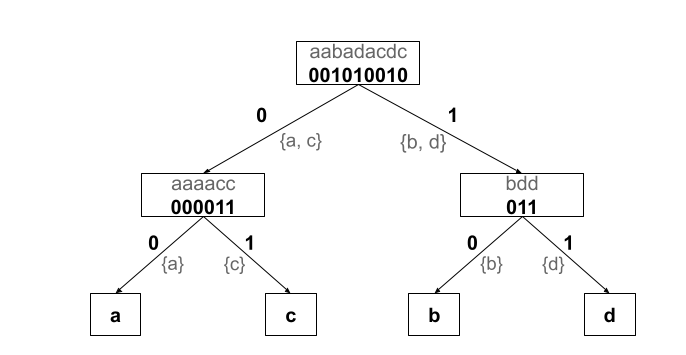
\includegraphics[width=0.9\textwidth, height=0.3\textheight]{images/wavelet_tree}
	}
	\caption[TODO]{Wavelet tree representation of text $S=\mathit{aabadacdc}$. We can see how
	the recursive partitioning of the alphabet works. In every node, we also show the
	subsequence represented (grey text) in the subtree of the node. The stored data can be
	recognized as they are in bold and black.
	}
	\label{obr:WaveletTreeExample}
	% based on https://simongog.github.io/assets/data/sdsl-slides/tutorial#23
	% source at https://docs.google.com/drawings/d/1cJyda3bdTluajr3iXu1x1iL5HF0JPZqAHw6jwct9KLI/edit
\end{figure}

On top of this, both $\rank_c$ and $\select_c$ methods on the original sequence can
be implemented using $\rank$/$\select$ methods applied on bit sequences that are along
the path from the root to the leaf containing character $c$. Thus, the number of
$\rank$ and $\select$ queries on individual bit vectors depends on the depth of
a leaf containing queried character $c$. It is possible for this representation to use
just $\BigO(\log \sigma)$ times more space than the single bit vector over this sequence as
on every level of the wavelet tree, we store in total a bit vector of length roughly $|S|$.

Even if this version of wavelet tree can be used inside of the FM-index, it is possible to
make a solution that is faster in some scenarios. Both methods, $\rank_c$ and $\select_c$ now
depend on the speed of the bit vector implementation, used in the nodes, but also on the depth
of symbol $c$ in the tree. This depth is now for every single character roughly $\BigO(\log \sigma)$.

To obtain a better solution, let us give another perspective on the wavelet tree and assign
single bit to every edge. For every edge, its bit is either {\tt 0} if this edge leads from
the parent to the left son or {\tt 1} otherwise. We can think of the wavelet tree as an assignment
of a binary code to every alphabet character. Code of a character $c$ in some leaf node is equal
to concatenation of bits that are contained in edges on a path from root to the leaf node.

The idea proposed by~\cite{makinen2005succinct} is to shape the wavelet tree in such a way that
a code of every character is equal to Huffman code of this character. The advantage we get is that
if queries for a characters are coming according to their frequencies, then we need to visit on average
only $\BigO(H_0)$ nodes rather than $\BigO(\log \sigma)$, where $H_0$ is zeroth-order empirical
entropy. It is defined as $$H_0(S)=\sum_{c\in\Sigma} \frac{\#_c(S)}{|S|} \lg \frac{|S|}{\#_c(S)},$$ 
where $\#_c(S)$ denotes number of occurences of symbol $c$ in $S$. Even if the maximum depth of the wavelet
tree may increase, \cite{grabowski2004first} showed that we can enforce the maximum depth to be $\BigO(\log \sigma)$
with the average depth limited by $H_0+2$. This is, however, not advisable in practice. The most
important fact is that with Huffman shaped wavelet tree, it is possible to decrease the average number
of nodes accessed and thus decrease the average query time of $\rank$ and $\select$.

The space used by the wavelet tree heavily depends on the space usage of individual bit vectors
that are used to store the nodes of wavelet tree. If these are represented using a data structure
that takes space close to the zero-order entropy of represented sequence, then the whole
wavelet tree requires $nH_0(S) + o(n\log\sigma)$ bits of space as was shown by \cite{grossi2003high}.

% TODO: FM-index vie zaberat H_k (+ citacia)

In this chapter, we presented some useful applications of the bit vector. We looked more closely on
FM-index, the data structure used for the problem of text indexing. There, we encountered the
problem of answering $\rank$ and $\select$ over the general alphabet and described wavelet tree,
one possible data structure that can be used to solve it, assuming we have an implementation of
bit vector supporting $\access$, $\rank$ and $\select$ methods.

\section{Outline of the Thesis}

The goal of this thesis is to describe current state of implementation of the bit vector
supporting $\access$, $\rank$ and $\select$ methods and come up with improvements that
make bit vector usable in more scenarios. This can be either by speeding up the current
implementations, saving some additional space but also by combination of these two as
obtaining some new ratios of query time and space used can also open doors to new applications.

In the second chapter, we show possible implementations of $\rank$ and
$\select$ methods. We discuss what are the theoretically optimal solutions but also
what are their practical drawbacks. We then proceed to describe one of the
widely used implementations of a compressed bit vector called \textit{RRR}.

In the third chapter, we propose our own modifications to the implementation of
a compressed bit vector based on RRR and we discuss theoretical aspects of these
modifications.

In the fourth chapter, we show our proposed implementation of previously devised
methods and experimentally test and evaluate them. We measure the performance
of our solution on artificial as well as real-world data. Finally, we demonstrate
how our idea can be used to get a better ratio of query time and space used by the
FM-index and thus deliver practically useful results.